\chapter{Background and Theory}

Vector graphics have been popular in the computer industry for many years,
seeing frequent use in analogue oscilloscopes, video arcade games \cite{astroids},
and as display devices for computers \cite{ibm2250}.

\section{Computer Graphics}
There are two different types of representing computer graphics today, vector graphics and raster graphics.

\subsection{Vector Graphics}
Vector graphics is a form of computer graphics where mathematical expressions are used to describe an image. The image, or the 'scene', is made up of primitives that describe paths, lines and curves, and sometimes combinations of these in order to create more complex shapes.

By relying on mathematical expressions instead of pixel values relative to screen resolution, vector graphics can be described as resolution independent. This is often conceptualized in the form of scaling: While scaling a rasterized image will result in a blurry image, scaling a vectorized image will result in the mathematical expressions being recalculated, and the image will remain sharp. This process is visualized in figure \ref{fig:vectorscaling}.

\begin{figure}[h!]
\centering 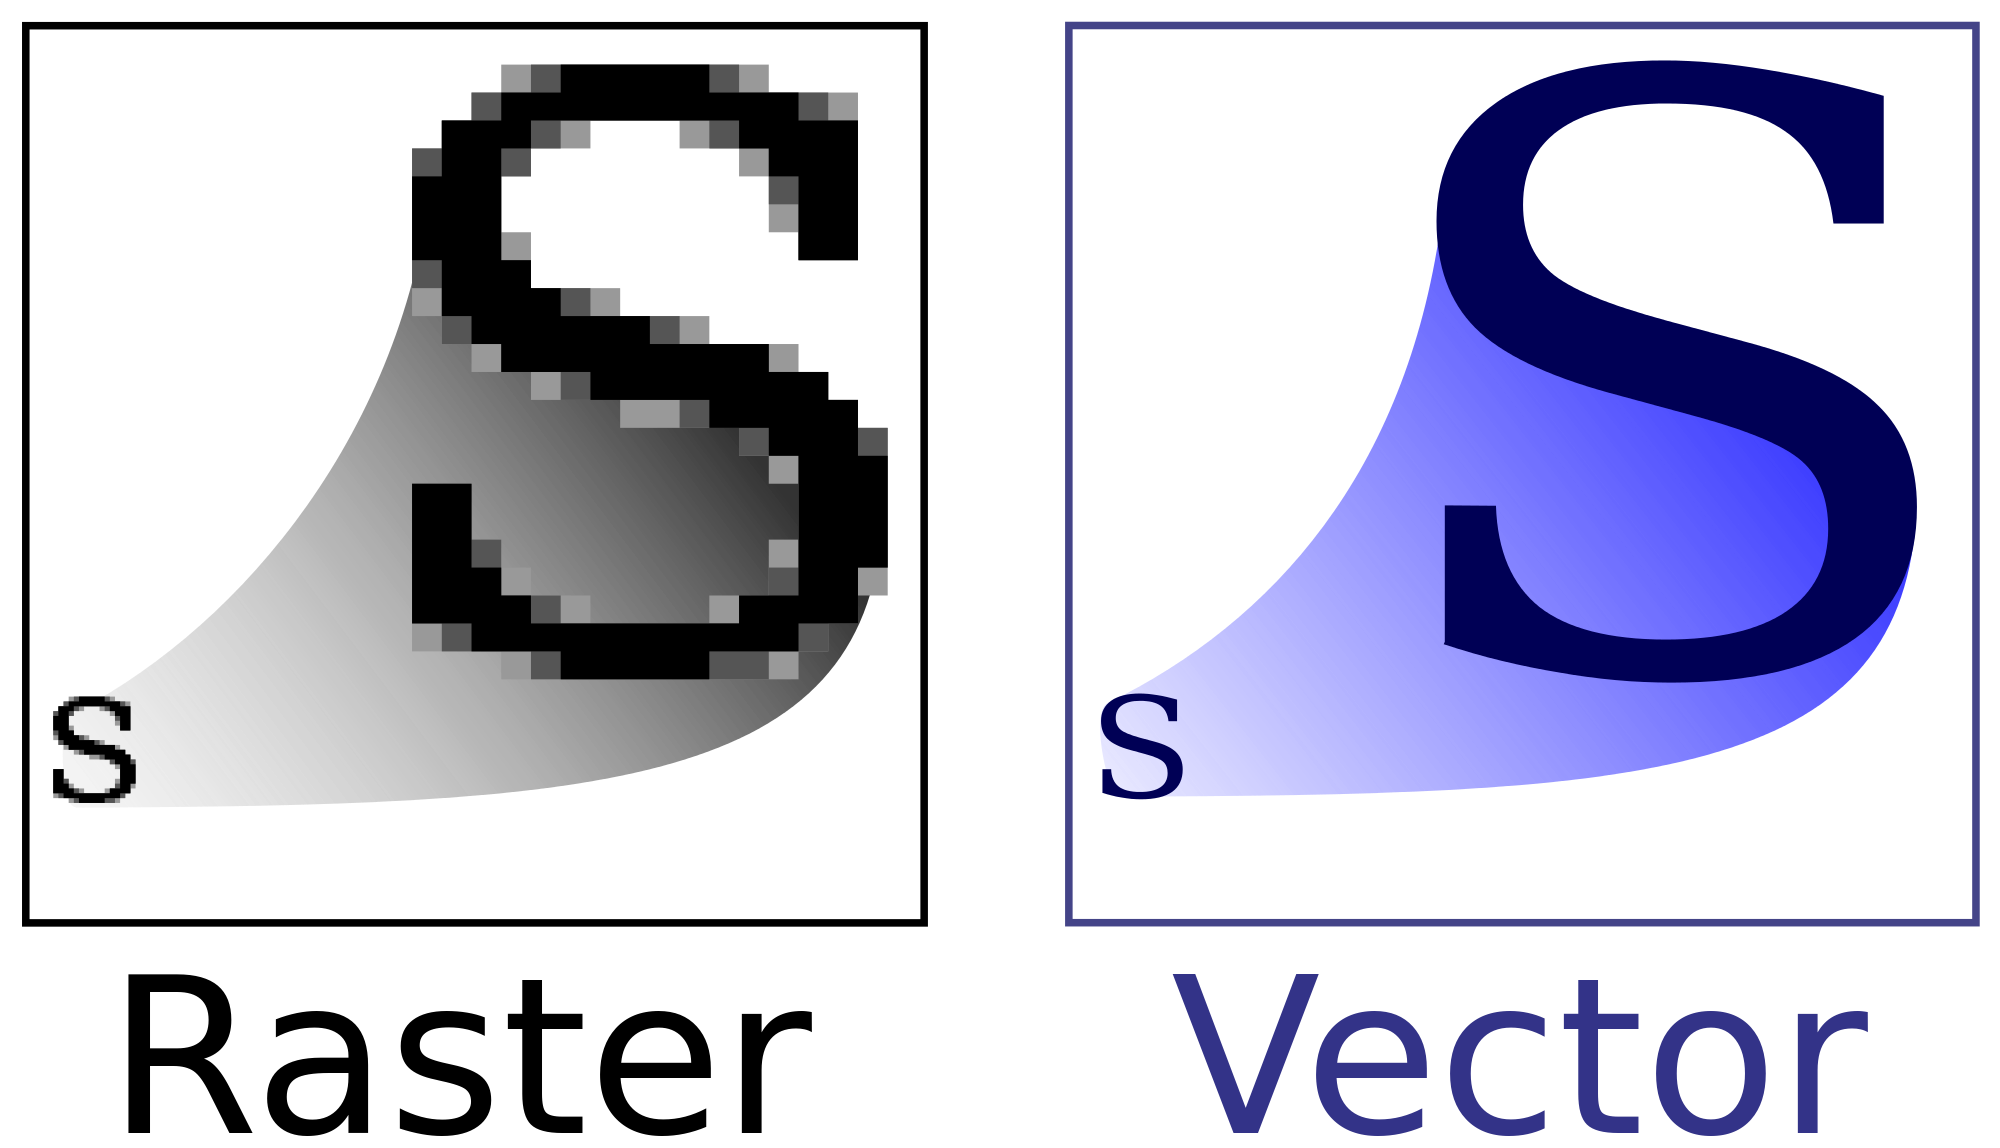
\includegraphics[width=0.5\linewidth]{images/bm_vs_svg.png}
\caption{Scaling comparison between raster graphics (left) and vector grahics (right). Source: \cite{svg}}
\label{fig:vectorscaling}
\end{figure}

Vector graphics are predominantly used to describe 2D graphics, in order to distinguish them from 2D raster graphics, which is described later on. In 3D graphics, most implementations utilize points, lines and curves to define shapes, which makes them a lot like vector graphics. Voxel graphics is an implementation of 3D graphics that tries to define it's shapes by utilizing three dimensional pixels, so-called 'voxels', but is rarely used.

Some computer font types, like TrueType uses vector graphics and more specifically Bézier curves to represent glyphs\cite{truetype}. // Is this necessary?

Due to the geometrical nature of vectors, it's not practical to use vector graphics to represent photographs. Computer generated text, drawings or imagery, for use in graphical design, is the most common use case for vector graphics today, since the graphic can easily be scaled up or down by demand. Most professional image processing and design software, e.g. Adobe Illustrator, support vector graphics. To store the graphics, file formats such as \texttt{.ai} (for use in Adobe Illustrator) or the open standard \texttt{.svg} (Scalable Vector Graphics) can be used.

Special types of monitors, called vector displays and described in the next section, are used to display vector graphics. Raster displays cannot display true vector graphics, and will need to rasterize them first.

\subsection{Raster Graphics}
Raster graphics is also known as bitmap graphics.
A raster image is a two-dimensional array of descrete values.
Each descrete value is used to describe the color of the pixel at a given position in the array.
A bitmap images is often represented by utilizing the RGB scheme.
RGB is a scheme where you define the amount of red, green and blue color of a pixel.

To display a full image, the computer needs to store \( (width \times height) \times RGB \) bits.
Today RBG usally contains 3 bytes, one byte for each color,
and a resolution of \(1920 \times 1080\) is becomming the standard.
A single image therefore requires about 6.2 MB to store.
There exists method to compress images, however raster images still uses a significant amount of space.


\section{Visual Display}
In the early days of computer display, vector displays were mainly used.
The use of frame buffers started when transistor-based RAM was introduced.
As a result raster graphics and displays were created \cite{graphics-visualization-algorithms}.
There exists vast variety of display technologies, a few examples are: CRT, LCD, LED and OLED.
Without going into detail about each technology,
a few of the basic principles will be described in the following subsections.

\subsection{Vector Displays}
A vector display/monitor displays graphics by drawing from point to point. 
All vector displays utilize CRT (Cathode Ray Tube) technology, which contain one or more electron emitters that fire electron beams that are deflected onto a phosphorescent screen to display images.

The basic vector display is monochromatic. 
However, certain displays with color support exist. 
By using a shadow mask - that is a perforated plate that acts as a filter - between the electron guns and the screen, different colors can be displayed. This is achieved by having one electron gun for red, green and blue. Each gun shoots electron at different angles through the mask, and different intensities for each gun can create different colors.

Vector displays are pretty much obsolete today, because of raster screens' inexpensiveness and support for graphics with a higher level of detail. 
Also, vector graphics can - with modern algorithms - efficiently be translated to raster graphics, called rasterisation.
Translating raster graphics to vector graphics, however, is a complex process.

// TODO: Maybe a few references for these statements?
\subsection{Raster Display}
There exists a variety of raster display technologies, however they have a few common attributes.

Raster graphics uses a tecnique called frame buffer.
A frame buffer is used to hold the current image.
When the screen is ready to read a new image, this is done from the frame buffer.
After the image has arrived, the images scanned line by line.
The scan is done from top to bottom of the image.


\section{Primitives}

// TODO: Introduce Bézier curves. Move whole section to solution.

The computer arcitechture supports 3 basic primitives: lines, quadratic Bézier curves and cubic Bézier curves.
Each primitive's type is identified by the 8 first bits.
To store a position on the screen, 32 bits is required: 16 bit for X and 16 bit for Y.
A line is represented by a start point and an end point.
To represent a quadratic Bézier curve a total of three points are needed, a start point, a control point and an end point.
The cubic Bézier curve includes one extra control point compared to the quadratic curve.
Table \ref{tbl:primitives} illustrates how each primitive is stored in the primitive buffer.
%A line start point is \(x_0 \) and \(y_0 \), and end point is \(x_1 \) \(y_1 \)

With the basic primitives line, quadratic Bézier and qubic Bézier all other shapes can be constructed.
E.g a rectangle is constructed by adding four lines together.

%\begin{center}
\begin{table}[h]
    \centering
    \label{tbl:primitives}
    \begin{tabular}{|l|l|l|l|l|l|l|l|l|l|}
    \hline
    Primitive type (8) & x (16) & y (16) & x (16) & y (16) & x (16) & y (16) & x (16) & y (16) & Total bits \\ \hline
    Line             & \(x_0 \)  & \(y_0 \)  & \(x_1 \)  & \(y_0 \)  & ~   & ~   & ~   & ~   & 72    \\ \hline
    Quadratic Bézier & \(p_0^x \) & \(p_0^y \) & \(p_1^x \) & \(p_1^y \) & \(p_2^x \) & \(p_2^y \) & ~   & ~   & 104   \\ \hline
    Qubic Bézier     & \(p_0^x \) & \(p_0^y \) & \(p_1^x \) & \(p_1^y \) & \(p_2^x \) & \(p_2^y \) & \(p_3^x \) & \(p_3^y \) & 136   \\ \hline
    \end{tabular}
    \caption{The table above shows how each primitive is stored in memory. Bit size in parenthesis.}
\end{table}
%\end{center}
